%\documentclass[11pt, a4paper]{article}

%\title{Ammonia Synthesis}
%\author{James Rhodes}
%\date{\today}

%\usepackage{fullpage}
%\usepackage{mhchem}
%\usepackage{setspace}
%\usepackage{inputenc}
%\usepackage{wrapfig}
%\usepackage{textcomp}
%\usepackage{graphicx}
%\usepackage{pdflscape}
%\usepackage{wrapfig}
%\usepackage{mathtools}


%\usepackage{graphicx}
%\graphicspath{ {graphics/} } 
%\linespread{1.5}



\newcommand\tc{400}
\newcommand\pbar{150}
\newcommand\ammOUT{227.6}  %daily average ammonia production requirement tonnes/day
\newcommand\conv{28}	%first pass conversion rate
\newcommand\purge{5}



%\begin{document}

%\maketitle
%\tableofcontents

%\doublespacing
\section{Ammonia Synthesis}
\subsection{Introduction}


\subsubsection{Overview}
The production process of ammonia is a key stage in converting the hydrogen gas produced in electrolysis and nitrogen from cryogenic separation of air into liquid ammonia. This is useful as it is significantly safer and cheaper to store long-term than hydrogen this is due to the significantly lower boiling point of hydrogen and thus the lower energy density of hydrogen at atmospheric conditions (2.96 MJ/L) compared to that of ammonia (13.77 MJ/L)\cite{Bartels2008} thus a not only would a volume 4.65 times greater than that of ammonia would be required for comparable energy storage. Significantly higher pressures and cryogenic temperatures would be required to store hydrogen in liquid form, making large quantities significantly more expensive to store.
\\
Stored ammonia can then be fed to the power generation side of the plant in order to match  the power demand of the region, and provide long term storage for renewable wind energy without the need for the combustion of fossil fuels.

In order to produce ammonia a reversible reaction takes place between hydrogen and nitrogen. The equation of reaction for ammonia synthesis from nitrogen and hydrogen is;

\begin{equation}
3H_2+N_2   \underset{ }{\stackrel{ }{\rightleftharpoons}}   2NH_3 \qquad \Delta h_0 = -92.44 \; kJ/mol 
\end{equation}

This synthesis reaction is exothermic and can be designed in such a way that the high temperature products of reaction can be used to preheat the reactants to the operating point of reaction in an auto-thermal process. This has significant benefits in terms of reducing the energy requirements of the plant. However, the process by which the reaction takes place can vary depending on the requirements of the plant.

\subsubsection{Design objective}
The ammonia synthesis stage of the plant design was required to meet the capacity of ammonia production for the storage of excess energy produced by the wind turbines. This can subsequently be stored as liquid ammonia and be used to generate electricity in the solid oxide fuel cell and gas turbine in order to match the fluctuating electricity demand of the region. A number of different methods of ammonia synthesis have been reviewed and considered in the design process in order to design a process best suited to the scale, technology, economic constraints and environmental impact of plant. 
\\
In regard to the scale, of the process an initial year long demand requirement for stored energy was calculated in the control and energy matching design process [REFERENCE WILL] this g both a requirement for the year-long average energy demand for stored ammonia as well as the maximum energy storage requirement cause by a supply/demand deficit. 
These requirements are shown in table \ref{req} below, using the known efficiencies of the power generation stages and their respective duties an annual demand for ammonia can be calculated. Supply-demand matching can also be used to calculate the maximum storage required throughout the year. This gives scale requirements for ammonia output and storage and thus the design requirements for my design process. 

As defined by the power demand of Maui, Hawaii the year average power is set to average at a plant output of $36.6MW$. Accounting for combined generation efficiency in the ammonia-to-power stage of $61.7\%$ this translates into a daily average ammonia output of $\ammOUT$ metric tonnes. However, this does not account for the variable supply of wind power and subsequent hydrogen. Thus the ammonia synthesis stage must be designed for a higher capacity to ensure that it can adjust to temporal fluctuations in energy supply. Thus a reactor with a capacity for $300$ tonnes per day will be designed with short term hydrogen storage and an an ammonia breakdown loop to ensure continuous operation of the synthesis process. 
\begin{table}[!htbp]
	\begin{center}
		\label{req}
		\caption{Design requirements of synthesis stage}
		
		\begin{tabular}{|c|c|c|c|}
			\hline
			Yearly output& Average output & Storage required & Power stage efficiency     \\ \hline
			83058 tonnes            & $\ammOUT $  tpd            & 15000 tonnes                          & 61.7 \%  \\ \hline
		\end{tabular}
		
	\end{center}
\end{table}


Further considerations were given to technological requirement, whilst new and emerging technologies were considered in the design process priority was given to methods that have been successfully implemented on medium and large scale processes, laboratory condition processes whilst considered were only chosen if there was a clear method in upscaling to industrial levels and the benefits of doing so were significantly greater than established industrial processes. This was due to the need for reliability of power supply, especially considering the island location of the power plant and the lack of alternative power sources.
Finally, consideration was given to the environmental and economic considerations. These were especially important if the plant was going to have to provide clear benefits over gas and coal power generation plants. Thus the impact of waste flows was considered heavily as was the opportunities to recycle materials where possible. 



\subsection{Review of ammonia synthesis methods}


\subsubsection{Haber process}
The most well established and widely used method for producing Ammonia is the process developed on an industrial scale in 1913 by Fritz Haber at BASF. This involved the reaction of N$_2$ and H$_2$ feed gases over a hetrogenous solid iron catalyst at high temperature and high pressure. The most common catalyst in this process is Fe in magnetite form. Whilst this process is well established and easily scalable with current production capacities exceeding 3000tpd \cite{Banares-alcantara2014} its low single pass conversion and large ramp-up time makes it difficult for demand matching, meaning the process is usually run as a continuous process. Despite this limitation a large number of research and improvements have been made to this process and with the addition of a recycle stream overall conversion rates above 95\% are now regularly achieved. Developments into the catalyst composition used in the reactor has led to lower pressure reactors and higher single pass conversion rates.

Perhaps the most significant of these has been the development of w\"{u}stite as an alternative to magnetite as the iron precursor in the catalyst. This has shown clear advantages in terms of ammonia first pass conversion at lower temperatures and pressures and for similar material promoters\cite{Pernicone2003} \cite{Liu1996}.


\subsubsection{Ruthenium-based synthesis}

A growing competitor to the iron-based synthesis route is an ammonia synthesis production route in which a Ruthenium based catalyst is used in place of the iron. Despite know usage in ammonia synthesis since 1917 it was not until 1972 that Ozaki et al demonstrated visibly higher activity in ammonia synthesis converters using Ru as an active component. This had led to field of research into its use as a catalyst and in 1992 the development of the KAAP (Kellogg Advanced Ammonia Process) industrial process for Ru-based ammonia synthesis \cite{Rossetti2006}. This process is typically able to operate under significantly lower pressures and feed ratios than iron-based catalysts, meaning a clear economic advantage in terms of reactor and pressure vessel design. The tradeoff is the scarcity of Ruthenium and thus the significantly higher cost of the catalyst. This can be shown in Table \ref{tab:cat} below \cite{Liu2014}.
{\renewcommand{\arraystretch}{1.4}
\begin{table}[!htbp]
	\begin{center}
	\label{tab:cat}
\caption{Comparison of ammonia synthesis catalysts}

	\begin{tabular}{|c|c|c|c|c|c|}
	\hline
	Catalyst& Availability & Cost (USD/m$^3$)* & T/ \textdegree C     & H$_2$/N$_2$ ratio & Energy consumption (Gj/t) \\ \hline
	Fe            & abundant              & 4750                          & 350-525 & 2-3             & $\sim$27                      \\ \hline
	Ru            & scarce                & 254100                        & 325-450 & under 2         & $\sim$27                      \\ \hline
\end{tabular}
{\small *converted from CNY data at March 2018 exchange rates}

\end{center}
\end{table}

The cost of Ruthenium being over 50 times greater than that of Iron is a huge factor in the cost of the reactor. Furthermore, the poisoning of the Ruthenium by high concentrations of hydrogen can mean the cost of replacing the catalyst.

\subsubsection{Electrocatalysis}
An alternate method of producing ammonia is to use electrocatalysis reaction. This is a non-spontaneous thermodynamic reaction:
\begin{equation}
3H_2O+N_2   \underset{ }{\stackrel{ }{\rightleftharpoons}}   2NH_3 + 1.5O_2 \qquad (K_{298} = 10^{-120})
\end{equation}	
This can occur using electric energy. This has shown similar efficiency to established synthesis methods under normal temperatures and pressures \cite{Liu2014}. In recent years this has been a growing field with research into materials for electro-catalysts and electrolytes. However, current limitations of low current efficiency and conversion rates make this technology one in need of further development. Despite this the process has some clear benefits, the main one being the use of water as a hydrogen source reduces the need for hydrogen production; enabling the direct conversion of  wind-generated electrical energy into ammonia.
{\begin{figure}[h]
		\centering
		\caption{Electrochemical ammonia synthesis - anode (l), cathode(r)  \cite{Kyriakou2017}}
		{\centering
			
			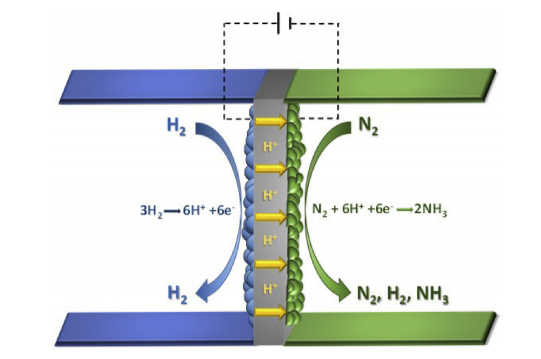
\includegraphics[scale=0.65]{electrochemical_synthesis}
			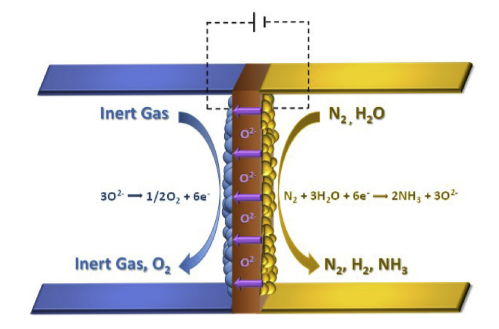
\includegraphics[scale=0.7]{electrochemical_synthesis2}	
	}
%source https://ac.els-cdn.com/S0920586116304138/1-s2.0-S0920586116304138-main.pdf?_tid=04f1f2e8-973d-448d-aadd-175ff2e8e895&acdnat=1523822193_0cdd35a3744e5241062382a77c9c5f63%
\end{figure}}



\subsubsection{Photocatalytic synthesis}
Using the same principles of photosynthesis the photocatalytic reaction of nitrogen and water to form ammonia and oxygen can be achieved at room temperature and atmospheric pressure under the addition of solar energy. However, despite ongoing research into this field and a number of photocatalysts available, the scale of this process would currently be unable to meet the ammonia requirement of the plant\cite{Liu2014}.


\subsection{Thermodynamic modelling}

\subsubsection{Equilibrium constant}

The equilibrium constant for ammonia synthesis was first calculated by Gillespie and Beattie (1930)\cite{Gillespie1930} and is a function of the reaction temperature.
\begin{equation}
logK_a = -2.691122log(T) - 5.519265\times10^{-5}T + 1.848863\times10^{-7}T^2+\frac{2001.6}{T}+2.6899
\end{equation}
{\begin{figure}[h]
\begin{center}

		\caption{Equilibrium constant K$_a$ of ammonia synthesis reaction at varying temperature}


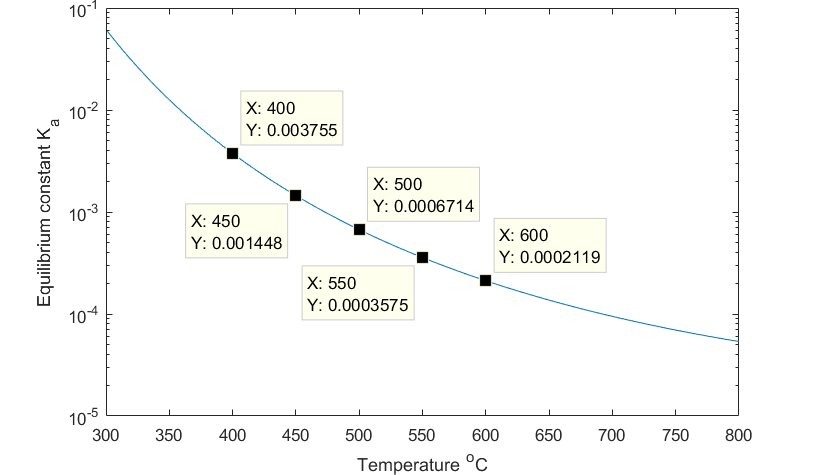
\includegraphics[scale=0.6]{K_a_varying_temperature}
\end{center}
\end{figure}}

This suggests that a lower temperature produces a higher equilibrium constant, as ammonia synthesis is an exothermic reaction theory supports this result as an exothermic reversible reaction favours the reactants as temperature increases.

\subsubsection{Reaction mixtures}
When calculating the properties of reaction mixtures throughout the system a rule of mixtures is used. Eqn. \ref{cpmix} gives the specific heat of a reaction mixture where $x_{i}$ are the mole fractions in the stream and $C_{p,i}$ are their respective specific heats. 
\begin{equation}
\label{cpmix}
	C_{p,mix} = x_{N_2}C_{p,N_2} + C_{p,H_2} + C_{p,NH_3}
\end{equation}
Calculating the respective specific heats  $C_{p,i}$ can be given by the polynomial temperature correlation Eqn. \ref{cp}.
\begin{equation}
\label{cp}
C_{p,i} = a + bT + cT^2 + dT^3
\end{equation}
\begin{table}
\caption{Specific heat coefficients \cite{Morgan2013}}
\label{cpco}
	\begin{center}
		 \begin{tabular}{|l|l|l|l|}
		\hline
			Coefficient & 
			N$_2$               & H$_2$               & NH$_3$              \\
			\hline
			a           & $28.9$               & $29.11$              & $27.568$             \\
			\hline
			b           & $-0.1571*10^{-2}$ & $-0.1916*10^{-2}$ & $2.5630*10^{-2}$  \\ \hline
			c           & $0.8081*10^{-5}$  & $10.4003*10^{-5}$  & $0.99072*10^{-5}$ \\
			\hline
			d           & $-2.873*10^{-9}$  & $-0.8704*10^{-9}$ & $-6.6909*10^{-9}$ \\
			\hline
		\end{tabular}
	
	\end{center}
\end{table}

\subsection{Mechanism and Kinetics}

\subsubsection{Reaction mechanism}

The reaction mechanism of the ammonia synthesis stage was key in understanding the kinetics of reaction and the effectiveness of a catalyst. This is due to the need for the $N_2$ bond to be broken on the surface of the catalyst during adsorption but also for the need for the dissociation of the bond during the synthesis step. The established mechanism steps for the ammonia synthesis reaction is understood to be the following reaction \cite{Jennings1991}.
\begin{subequations}
	\label{mech}
\begin{align}
H_2+*   &\underset{ }{\stackrel{ }{\rightleftharpoons}}   2H_{ad}\\
N_2+*   &\underset{ }{\stackrel{ }{\rightleftharpoons}}   N_{2,ad}\\
N_{2,ad}   &\underset{ }{\stackrel{ }{\rightleftharpoons}}   2N_{ad}\\
N_{ad}+H_{ad}   &\underset{ }{\stackrel{ }{\rightleftharpoons}}   NH_{ad}\\
NH_{ad}+H_{ad}   &\underset{ }{\stackrel{ }{\rightleftharpoons}}   NH_{2,ad}\\
N_{2,ad}+H_{ad}   &\underset{ }{\stackrel{ }{\rightleftharpoons}}   NH_{3,ad}\\
N_{3,ad}   &\underset{ }{\stackrel{ }{\rightleftharpoons}}   NH_{3}+*
\end{align}
\end{subequations}
Where $*$ denotes the forming of an adsorption site. Experimental studies have found the adsorption of nitrogen (\ref{mech}b) to be the rate determining step in this process and thus leading to an understanding of the microkinetics of the rate of reaction. This is due to the strong N$_2$ triple bond that must be broken.

%As the reaction is exothermic an increase in temperature would favour the reactants over the products. Experimental studies have confirmed this. The equilibrium constant $K_a$ can be found using the Gillespie and Beattie equation;
%


\subsubsection{Rate of reaction}

Numerous models \cite{Aparicio2008} for the rate of reaction of ammonia synthesis, however, the most widely used model for the rate of reaction is the Temkin equation \cite{Guacci1977}. Whilst a number of different forms of the equation have now been developed the Dyson and Simon \cite{Dyson1968} form is preferred in this analysis due to its simplicity and the limited experimental data required to simulate results.

\begin{equation} r_{NH_3} = K_2 \left [ K_a^2 \times f_{N_2}
\left ( \frac{f_{H_2}^3}{f_{NH_3}^2} \right ) ^\alpha - \left ( \frac{f_{NH_3}^2}{f_{H_2}^3} \right ) ^{\alpha - 1}
\right ]
\end{equation}

This equation the fugacities, $f$, rather than partial pressures have been used. Whilst the values of the equilibrium constant $K_a$ is well known the constant of reverse reaction $K_2$ and empirical constant $\alpha$ are found experimentally.

{\begin{figure}[h]
		\centering
		\caption{Reaction rate of ammonia synthesis}
		{\centering
			
			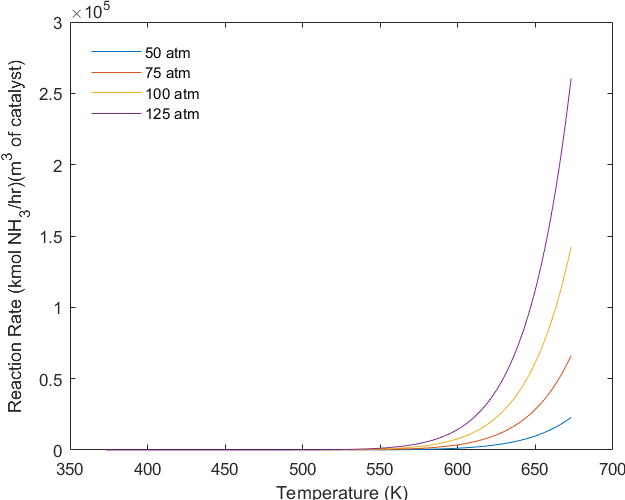
\includegraphics[scale=0.474]{reactionrate}
			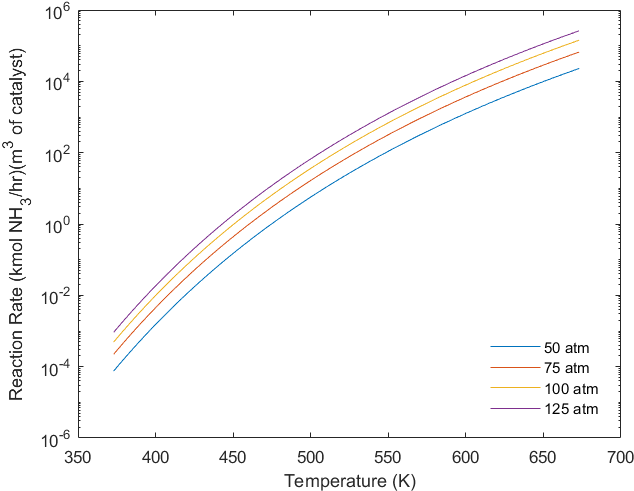
\includegraphics[scale=0.474]{LOGreactionrate}	
		}

\end{figure}}


This it is clear that as temperature and pressure inside the reactor increases the rate of reaction also increases. However, whilst the rate of reaction is known to increase within the reactor the equilibrium constant of reaction moves further towards the reactants due to the exothermic nature of reaction. 

Furthermore due to the NH$_3$ fugacities appearing in the denominator in both terms of the rate equation the equation breaks down when no ammonia is present clearly this does not follow the thermodynamic principles of a reverse reaction. Thus for the purpose of modelling a trace amount ($\leq$1\%) of ammonia was included in the initial reactants. As the reactor will be run at steady state reaction is analysed. 

\subsubsection{Fugacities}
The fugacities of the respective gases can be calculated using


\begin{table} [!htbp]
	\begin{center}
\begin{tabular}{ p{5cm}p{3cm} }
$f_N{_2}= P\gamma_{N_2}\frac{a}{3\delta}(1-b_2Z)$& $a= \frac{3\delta}{3+ 1}$\\
$f_H{_2}=P\gamma_{H_2}a(1-b_1Z) $&$ b_1 = \frac{i_0 +0.5 + (0.5/\delta)}{1-i_0}$\\
$f_NH{_3}=P\gamma_{NH_3}\times Z $&$ b_2 = \frac{i_0 - 0.5 +1.5\delta}{1-i_0}$ \\
\end{tabular}
\end{center}
\end{table}

Fugacity coeffiecients $\gamma$ can be calculated using the Cooper (1967) and Newton (1935) expressions given below;
\begin{equation} 
\gamma_{N_2} = 0.93431737 + 0.3101804\times10^{-3}T+0.295896\times10^{-3}P-0.2707279\times10^{-6}T^2+0.4775207\times10^{-6}  P^2
\end{equation}
\begin{equation} 
\gamma_{H_2} = exp\{ e^{(-3.8402*T^(0.125)+0.541)}P-e^{(-0.1263*T^(0.5)-15.980)}P^2+300*[e^{(-0.011901*T-5.941)}](e^{(-P/300)}-1)\}
\end{equation}
\begin{equation} 
\gamma_{NH_3} =0.1438996 + 0.2028538\times10^{-2}T - 0.4487672\times10^{-3}P - 0.1142945\times10^{-5}T^2 + 0.2761216\times10^{-6}P^2
\end{equation}
The sensitivity of the fugacity coefficients to temperature can be seen on figure \ref{fugco}. Showing that as temperature decreases and pressure increases the behaviour of gases becomes increasingly non-ideal. 
{\centering
	\begin{figure}[h]

		\caption{Variation of fugacity coefficients with temperature}
		\label{fugco}
			
			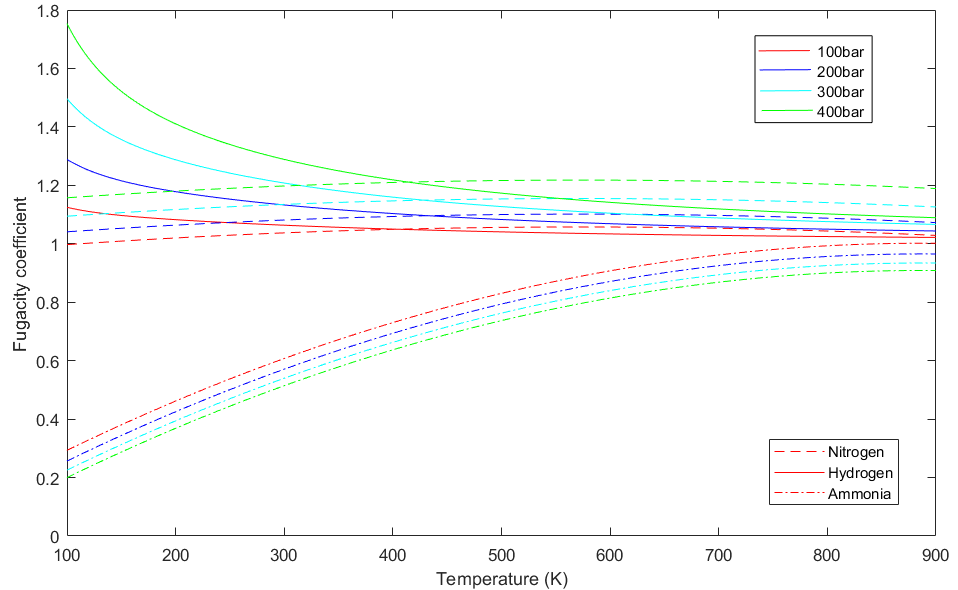
\includegraphics[scale=0.65]{fugacity_coeff}
		
\end{figure}}

\subsubsection{Modelling}
When modelling this Kinetic model and implementing the design into ASPEN a Langmuir-Hinshelwood –Hougen-Watson (LHHW) kinetic model, simulating the model using the surface mechanisms during the reactions. This is most commonly used when modelling heterogeneous reactions with a solid catalyst and fluid reactants. To simulate this model using ASPEN the general form of the model must be given \cite{Plus2008};
\begin{equation} 
Rate = \frac{(Kinetic factor)(Driving force)}{(Absorption)}
\end{equation}


In this form and using the Dyson and Simon form of the Temkin equation we can set the absorption term to unity and the kinetic factor to $k_{2}$, giving a driving force expression; 
\begin{equation} Driving force = K_a^2 \times f_{N_2}
f_{H_2}^{3\alpha}f_{NH_3}^{-2\alpha} - f_{NH_3}^{(2\alpha-2)}f_{H_2}^{(3-3\alpha)} \end{equation}

Using the experimental values for $k_20$ and $E^2$ in the Arrhenius law to calculate $k_2$ and then the Gillespie and Beattie equation to calculate $K_a$ and an experimental value of $\alpha = 0.5$ a kinetic model for the reaction was formed. Initial simulations of this model in a PFR reactor in aspen at a first approximation of industrial conditions (p=100bar T=400\textdegree C) gave an first pass conversion of $\approx25\% $ NH$_3$ first pass conversion.

\subsection{Catalyst}

In modelling the rate of reaction Dyson and Simon accounted for the flow of reactants through a reactor. In order to account for the presence of a solid catalyst an effectiveness factor $\xi_{c}$ was used such that an effective rate ($r_{eff}=\xi_{c}r_{NH_3}$) through the reactor could be calculated using the following assumptions\cite{Dyson1968}; The catalyst particles can be considered as spheres. The diffusion coefficients of each component are independent of position within a particle, Isothermal particles, Knudsen diffusion is not experienced. Giving the equation;
\begin{equation}
	\xi_{c} = \frac{(\text{molar flux of componenet i across surface})\times(\text{surface area of catalyst pellet})}{(\text{vol. of catalyst pellet})\times(\text{rate of formation of component i at surface comp.,T,P})}
\end{equation}

Throughout the past 100 years of an Fe-based magnetite (Fe$_{2}$O$_3$) precursor with a variety of oxidic promoters have been the principal catalyst used industrially in ammonia synthesis \cite{Liu2014}. However, over the past few decades a number additional catalysts have been developed. These involve the use of a various other materials as promoters including ruthenium and bimetallic nitrides, these were considered during the initial design of the plant due to their higher yields of ammonia at reduced pressures. This was mainly due to both the high cost and limited availability of Ruthenium. Considering the island location of the power generation facility the availability of resources was a key factor in the choice of catalyst.

On balance, the additional cost of these materials are substantially higher than iron and thus greatly increase both the initial capital costs of the plant but also the running costs of the plant due to the increased material costs. Thus an alternative w\"{u}stite (Fe$_{1-x}$O) iron catalyst was chosen for the ammonia synthesis stage. This was chosen due to the increased reaction rate at lower operating pressure than the traditional magnetite promoter thus reducing the pressure needed for the reactor and thus the capital costs required. The catalyst in use will be the A301 catalyst manufactured by Shangyou Catalyst Co. Ltd. 



\begin{table}[!htbp]
\begin{center}
\caption{A301 Catalyst composition}
\begin{tabular}{ |p{3.5cm}|p{2.05cm}|  }

	\hline
	Compound & Wustite (\%)\\
	\hline
	Fe oxide (Precursor) & 93\\
	\hline
	Al$_2$O$_3$ (Promoter)&   2.7\\
	\hline
	K$_2$O (Promoter)&0.8 \\
	\hline
	CaO    (Promoter)&2.8 \\
	\hline
	Others*& 0.7\\
	\hline
		\multicolumn{2}{|c|}{*Impurities in raw material} \\

	\hline
\end{tabular}
\end{center}
\end{table}

In the case of catalyst particles 


\begin{table}[!htbp]
	\begin{center} 
	\caption{W\"{u}stite catalyst properties \cite{Pernicone2003}}
	\begin{tabular}{ |p{4cm}|p{3cm}|  }
	\hline
	A301 particle size & 0.15-0.25mm\\
	\hline
	Bulk density & 3.25 g/cm$^3$\\
	\hline
	BET total surface area & 16.6 m$^2$/g\\
	\hline
	K$_{20}$&  0.874 x 10$^{16}$\\
	\hline
	E$_2$ &44.9 kcal/mol \\
	\hline
	

	\end{tabular}
	\end{center}
\end{table}


\subsection{Reactor design}
The synthesis reactor is central to the design of the process as it is within here that the synthesis reaction takes place. In order to maintain close to optimum conditions within the reactor I have chosen to separate my reactor into two beds with intercooling between them. This enables the products of the first bed to return to a lower temperature before entering the second stage.

{\begin{figure}[!htbp]
		\caption{Reactor stage with integrated heat exchanger}
		
		\centering
		
		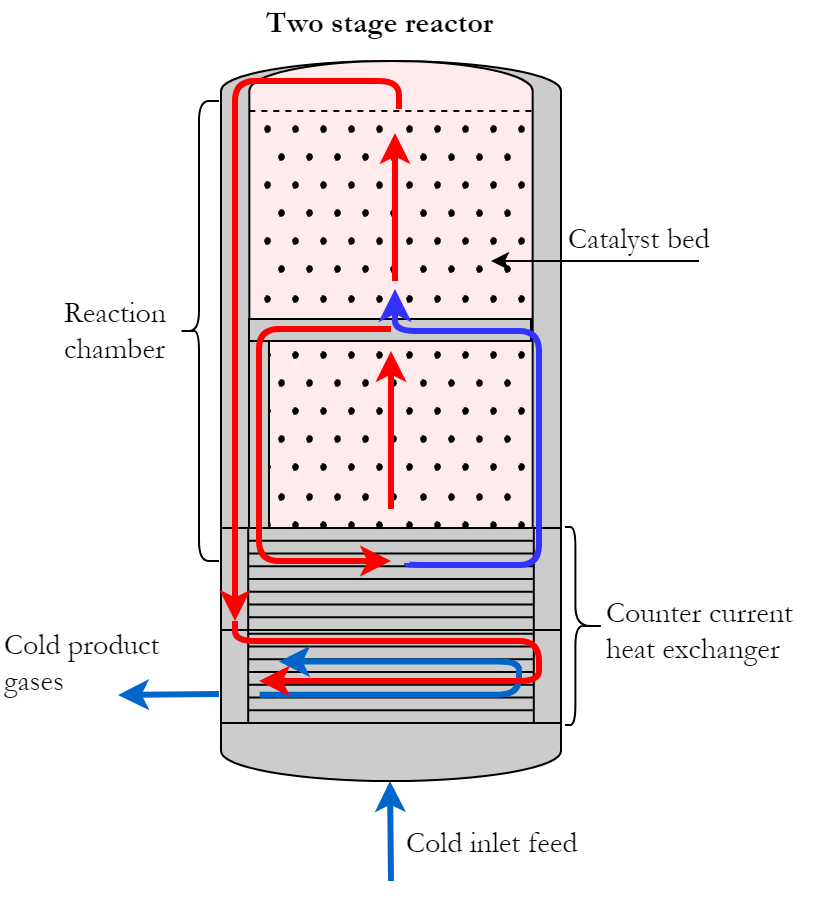
\includegraphics[scale=0.3]{twostage_reactor}
	\end{figure}
}

\subsubsection{Reactor sizing}
The reactor consists of two reactor stages with interstage indirect cooling. Both reactor inlet stages are designed as fixed bed reactors with an even catalyst spacing throughout. Modelling the outlet temperature against reactor length in figure \ref{Rlen} for a single bed with an input temperature of 400 \textdegree C and a diameter of 0.2m shows a change in the reactor profile up to L=0.25m after this point increasing the reactor length no longer increases the NH$_3$ yield thus this was chosen as a suitable length for the first stage. Using this first stage design a second bed could be subsequently designed. Using a larger bed was required to optimise ammonia yield. Simulating the reactor bed on ASPEN an optimum length of D=0.25m and L=0.9m was chosen as after this point there was no significant increase in performance with reactor length, giving a first pass conversion of 35.2\%.\cite{Elnashaie1989}

{\begin{figure}[!htbp]
		\caption{First and second reactor temperature and yield profile with length}
		\label{Rlen}
		\centering
		
		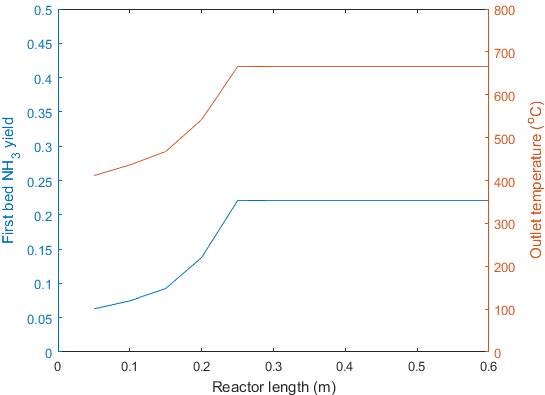
\includegraphics[scale=0.5]{reactorlength_profile1}
		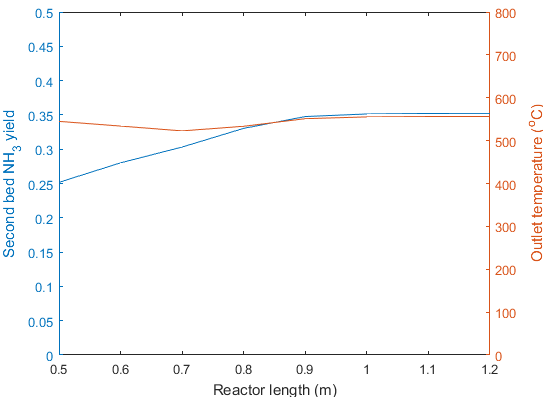
\includegraphics[scale=0.5]{reactorlength_profile2}
	\end{figure}
}


Furthermore, under a reactor pressure of \pbar  bar the thickness of the walls must be sufficient to withstand the high internal pressures of reaction.
\subsubsection{Material selection}
In order to calculate the thickness of material required  the internal reactor forces must be measured. As must the operating temperatures. From my simulation the peak temperature of normal operation of the reactor remains below 700\textdegree C. Therefore assuming a material with a melting point significantly higher than this would be required. Due to the corrosivity of NH$_3$ to a number of metals high-yield steel was chosen as the material for construction of the vessel. 
\begin{table}[!htbp]
	\begin{center}
		\label{req}
		\caption{Properties of high yield steel \cite{Howatson1972}}
		
		\begin{tabular}{|c|c|c|c|c|}
			\hline
			Density& Melting point & Yield stress & Ultimate tensile strength& Cost    \\ \hline
			7850 kg/m$^3$       & 1500\textdegree C          & 400 MPa                          & 600 MPa&\$896/tonne \cite{Meps2018} \\ \hline
		\end{tabular}
		
	\end{center}
\end{table}

To ensure the reactor material can withstand the reactor pressures it must both withstand the hoop and longditudinal stresses within the reactor such that.
\begin{equation}
\frac{\sigma_{yield}}{S.F.} \geq \sigma_L=\frac{PD}{4t} \text{  and  } \frac{\sigma_{yield}}{S.F.} \geq \sigma_H=\frac{PD}{2t}
\end{equation}
Where a safety factor of 2 is taken. This gives the condition that for high yield steel t$\geq9.375mm$. Thus taking the thickness of the vessel is taken to be 10mm. This gives a volume of steel required of 10.75dm$^3$ at a  combined mass of the two steel vessels to be 84.39kg without a catalyst bed present.

CHECK LEAK BEFORE BREAK CONDITION
\subsubsection{Pressure drop}

Pressure drop across a reactor can be calculated using the Ergun equation \cite{Ergun1949}

\begin{equation}
	\frac{\Delta p}{L}= \frac{150\mu(1-\epsilon)^2}{D_p^2\epsilon ^3}v_s+\frac{1.75(1-\epsilon)\rho}{D_p\epsilon ^3}v_s^2
\end{equation}
Where $\Delta p$ is the pressure drop across the length $L$ of the bed, $\mu$ is the fluid viscosity, $\epsilon$ is the void space in the bed (taken as $\epsilon = 0.5$ \cite{Ergun1949}), $\rho$ is the density of the fluid, $D_p$ is the particle diameter and $v_s$ is the superficial velocity of the fluid where $v_s = \frac{Q}{A} = \frac{\text{volumetric flow rate}}{\text{bed cross sectional area}}$.
\begin{table}[!htbp]
	\begin{center}
		\caption{Reactor dimensions and pressure drop}
			\begin{tabular}{ |p{2.3cm}|p{2.3cm}|p{2.3cm}|p{2.3cm}|p{2.7cm}|p{2.3cm}| }
				\hline
				
				Reactor bed & Volume (m$^3$)& Length (m)&Diameter (m)&Thickness (mm)&$\Delta p$ (atm)\\
				\hline
				 1&0.00785 & 0.25 &0.2 &10.0& \\
				\hline
				 2&0.04418 & 0.9 &0.25 &10.0&\\
			
				\hline
			\end{tabular}
	\end{center}
\end{table}
\subsubsection{Heat exchanger}

For my two stage reactor design intermediary cooling was a key factor in ensuring that the exothermic synthesis reaction did not result in an unwanted temperature increase, thus shifting the equilibrium of reaction further towards the reactants. There were two main methods considered in literature. These were direct quench cooling and heat exchanger indirect cooling.

\subsubsubsection{Quench cooling}
Direct quench cooling involves the addition of cold feed mixtures during the reactor stages in order to reduce the reactor temperature at each stage. This means that only a fraction of the total feed enters the first reactor stage.
\subsubsubsection{Indirect cooling}
Indirect cooling involved a heat exchanger passing the hot product gases past the cold feed gases in order to raise the temperature of the feed gases. This means the entire feed stream passes through all reactor stages and thus the time in the reactor is maximised.
\subsubsubsection{Design}
The chosen method for cooling configuration was the indirect cooling method due to the maximisation of reaction time. This is supported by empirical analysis \cite{Penkuhn2017}. The heat exchanger used in the reactor is a counter-current heat exchanger with steady state heat transfer. From this it is possible to derive an energy balance equation \cite{Jinasena2016};
\begin{equation}
\frac{dT_c}{dx}=\frac{UA}{\dot m_i C^i_pL}(T_h-T_c)  
\end{equation}
\begin{equation}
\frac{dT_h}{dx}=\frac{UA}{\dot m_o C^o_pL}(T_h-T_c)
\end{equation}
In which $T_c$ and $T_h$ are the respective cold inlet and hot outlet streams.$A$ is the area for heat transfer to occur and $U$ is the overall heat transfer coefficient of the heat exchanger (290.35Wm$^{-2}K^{-1}$)\cite{Elnashaie1988}, whilst $C_p$ are the specific heat capacities for the respective inlet and outlet streams of gas mixtures (Eqn. \ref{cpmix}) and $\dot m$ are the mass flow rates of the respective streams. Along a heat exchanger of length $L$ where $x$ is the relative position along it. If we then assume that assuming $\dot m_i c^i_p$ is equal to $\dot m_o c^o_p$ and similarly $\frac{UA}{\dot m_i c^i_p}$ does not depend on $x$. Then we can simplify the above expressions in order to give the temperature at the reactor inlet;
\begin{equation}
T_r^i = \frac{T_i + \frac{UA}{\dot m_i C^i_p}T_r^o}{1+\frac{UA}{\dot m_i C^i_p}}
\end{equation}
Similarly for the outlet of the heat exchanger
\begin{equation}
T_o = \frac{T_r^o + \frac{UA}{\dot m_i C^i_p}T_i}{1+\frac{UA}{\dot m_i C^i_p}}
\end{equation}

The aim of the heat exchanger is twofold. The first of these is to heat up the feed of the product gases to a significantly high temperature to allow for a suitable rate of reaction. This is done by running the hot product gases in counter current to the feed gases. The second use of the heat exchanger is in a two-stage reactor system the heat exchanger acts as an intermediary coolant for the product gases. This brings the temperature down to one in which the reaction equilibrium maintains a increased fraction of ammonia products.

\subsection{Additional units}

\subsubsection{Separator}
In order to remove the fraction of ammonia from the product mixture the relatively high boiling point of ammonia was used to remove liquid ammonia at high pressure and low temperature in a separator. This separates liquid droplets from gas particles by using gravity separation to allow the gaseous products to leave from the top outlet whilst liquid ammonia is removed from the bottom outlet in a vertical separator.

To separate liquid ammonia from the product gases I have used the Souders-Brown design equations to equate the drag force $F_D$ exerted by gas flow to the gravity force of the droplet weight $F_G$ \cite{Campbell2015} \cite{Jekel2001}. Such that assuming plug flow $F_D = F_G$. Substitution of expressions for the forces on a spherical droplet give the Souders-Brown expression \cite{Souders1934};
\begin{equation} V_{Gmax}=K_s\sqrt{ \left ( \frac{\rho_L - \rho_G}{\rho_G} \right )}\  when \  K_s = \sqrt{ \left ( \frac{4gD_P}{3C_D} \right )} \end{equation}

\begin{equation}D_{min} = \sqrt{\left ( \frac{(4/\pi)q_a}{F_GV_Gmax} \right ) } \end{equation}
\\ 
Where K$_s$ is found experimentally. Using a high mist extractor - a horizontal wire mesh pad in a vertical separator used to coalesce the liquid into droplets large enough to drop from the mesh pad gives $K_s = 0.12$. For a length/diameter ratio of 3/1 to reduce the material required in construction. And using a industrial standard XXX steel the separator can be modelled as a thin walled pressure vessel to calculate the required wall thickness of the tank.
\begin{equation}
	\sigma_{yield}=\frac{pr}{t}
\end{equation}
For an internal pressure of 140bar, known material and dimensions the separator can be sized.

{\begin{figure}[h]
		\caption{Vertical separator with mist extractor}
		
		\centering
		
		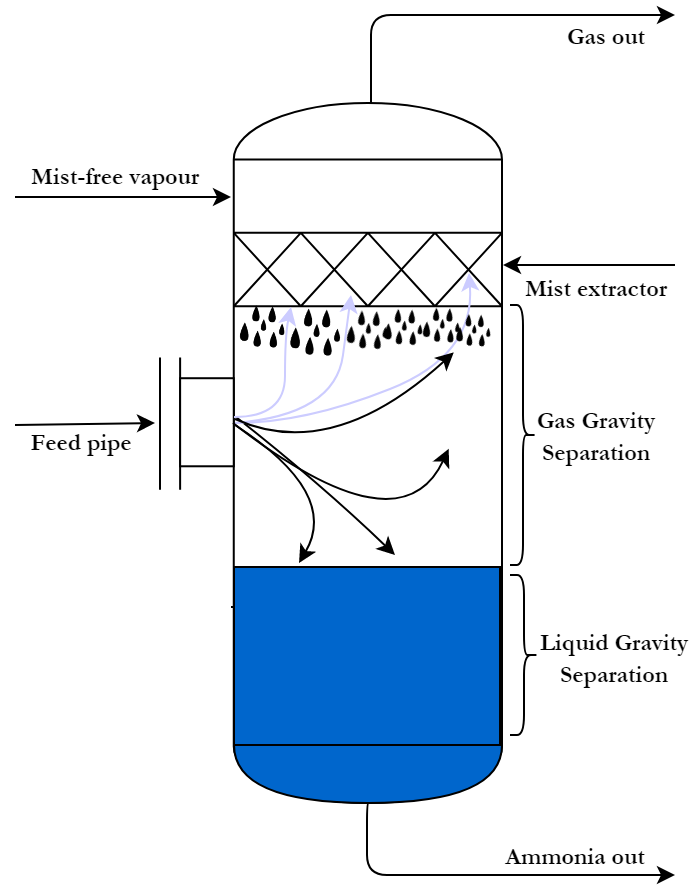
\includegraphics[scale=0.3]{ammonia_condenser}
	\end{figure}
}

\subsubsection{Compressor}
In order to obtain the high operating pressures required for ammonia synthesis centrifugal compressors are used both in the feed streams and in the reactor inlet stream. The feed stream is used to raise the pressure of the new feed to the pressure of the recycle stream whilst the reactor inlet the stream the recycle/feed mix is compressed to raise the pressure to account for the pressure drop of reaction. In this analysis we can assume that the compressors are driven by electric motors, however, turbine powered compressors are also possible; had the gas turbine generator been run continuously for power generation this would also have been considered. 
For an isentropic compressor the total output temperature can be calculated from Eqn. \ref{compT} \cite{Morgan2013}.
\begin{equation}
\label{compT}
T_{out} = T_{in}\left[ \left( \frac{P_2}{P_1}\right)^{\frac{1}{N}} \right]^{\left( \frac{n-1}{n}\right)} 
\end{equation}
The total 
compression power required $\dot W_{fluid}$ for the fluid is given by Eqn. \ref{compP}
\begin{equation}
\label{compP}
\dot W_{comp} = \frac{ \dot W_{fluid}}{\eta_{comp}} = \frac{1}{\eta_{comp}} TN\frac{n}{n-1}R\dot m \left( \left[ \left( \frac{P_2}{P_1}\right)^{\frac{1}{N}} \right]^{\left( \frac{n-1}{n}\right)} - 1 \right)
\end{equation}
Where $T$ is the input temperature, $N$ is the number of compressor stages, $n$ is the polytropic exponent, $R$ the specific gas constant, $\dot m$ is the mass flow rate and $P_1$ and $P_2$ are the respective inlet and outlet pressures. $\eta_{comp}$ is the overall compressor efficiency which the product of mechanical and isentropic efficiencies such that $\eta_{comp} =\eta_{is}\eta_{m}$. Standard efficiences of centrifugal compressors are taken as $\eta{is} = 0.85$ and $\eta_m = 0.95$ REFERENCE HERE. 

\subsubsection{Purge}
In order to limit the build up of inert gases within the synthesis loop a fraction of the recycle loop is purged. However, due to the cost of obtaining feed gases it is beneficial to keep the purge fraction small. After simulating a number of purge fractions on ASPEN a fraction of \purge \%  of the recycle stream was chosen. This purge stream is comprised of mostly H$_2$ and N$_2$ feed gases. Considering the high energy requirement of the electrolyser hydrogen recovery of this stream is in both environmental and economic interest. For this stage there are two main methods; membrane technology and cryogenic separation. With the former generally requiring a lower initial investment whilst the latter provides a greater energy efficiency \cite{Ojha2010}. In the initial 

In order to fu
\subsection{Optimising operation and control}
\subsubsection{ASPEN simulation}
\newpage
\subsubsection{Plant control}
\newpage


\subsection{Ammonia storage}
Storage of liquid ammonia product the main method in which the supply and demand sides of the plant are matched. Thus the scale of this storage must be one of the largest stores in the plant. Liquid ammonia has a boiling point of -33.3\textdegree C at atmospheric conditions, however, this can be increased by pressure storage. This requires a compromise to me made between low temperatures and high pressures in which to store ammonia. A review of current large-scale ammonia storage methods (Bartels,2008)\cite{Bartels2008} with the main trade-off between high pressure and low temperature storage being the high capital cost of building high pressure vessels against the increased energy requirements and thus running costs of maintaining low temperature storage. 
\subsubsection{High pressure storage}
Does not loose any required fuel, does not require energy to maintain. Limited by material used for the pressure vessel. So to increase capacity more vessels would be required. Bartels calculates that to store ammonia at an ambient temperature of 20$^o$C a pressure of 8.58 bar would need to be maintained. However, the limiting size of a steel pressure vessel is calculated to be approximately 270t. The recommended ratio is about 2.8ton NH$_3$ stored for every tonne of steel. 
\subsubsection{Low temperature storage}
Storage a of NH$_3$ at low temperature and ambient pressure is commonly used for large scale storage due to higher ammonia/steel ratio and thus a reduction in capital cost. At atmospheric pressure approximately 43 tonnes of ammonia can be stored per tonne of steel. This massively reduces the capital cost on steel. Despite this other factors must also be considered, the main on being the boil-off rate of liquid ammonia due to heat transfer from the environment. This is typically below a conservative estimate of 0.1\% per day \cite{Belapurkar2016}. This can then be captured and re-condensed at a total efficiency of 93.6\% [INSERT SOURCE] using an ammonia refrigeration cycle system 
{\begin{figure}[h]
		  \caption{Cold NH$_3$ storage cycle}
		
	\centering
	
	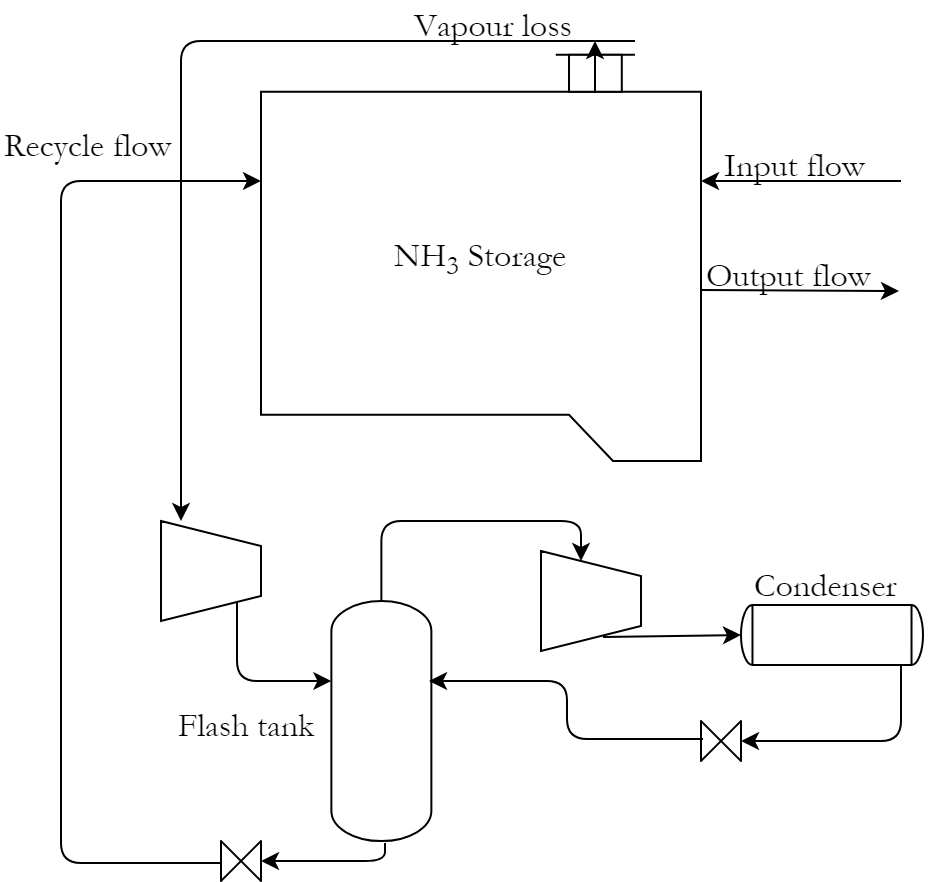
\includegraphics[scale=0.3]{ammonia_storage1}
\end{figure}
}
For a 15000 tonnes of ammonia storage a storage tank of at least $21.997\times10^3$ m$^3$ would be required (density of liquid ammonia, $\rho_{NH_3(l)}$=681.9 $kg/m^3$)\cite{Hacker2003}. 
\subsubsection{Design}
As calculated in [REFERENCE THE DEMAND/SUPPLY PROFILING] the maximum capacity for required ammonia storage is calculated to be 15000 tonnes at maximum capacity. Due to the scale of the process this would require at least 55 pressure vessels with over 5000 tonnes of steel.

\begin{table}[!htbp]
	\begin{center}
	\caption{Ammonia storage methods}
\begin{tabular}{ |p{5cm}||p{3cm}||p{3cm}|| }
	\hline
	\multicolumn{3}{|c|}{Ammonia Storage - 15000 tonnes required } \\
	\hline

	Properties & High pressure& Low temperature\\
	\hline
	NH$_3$ Energy density (MJ/L) & 13.77& 15.37\\
	Ammonia/Steel ratio & 2.8& 43\\
	Pressure required (bar) & 8.58 &Atmospheric\\
	Temperature required ($^o$C)& 20 &-33.3\\
	Storage efficiency&100\%&96.3\% \\
	
	Tanks required   &55&1 \\
	Steel required (tonnes)   &5357&349 \\
	Capital cost* (\$ m)   &4.800&0.3127 \\
	
	
	\hline
\end{tabular}
\\
{\small
	*Cost of steel at \$896/tonne \cite{Meps2018}}
\end{center}

\end{table}

%https://lib.dr.iastate.edu/cgi/viewcontent.cgi?referer=https://www.google.co.uk/&httpsredir=1&article=2119&context=etd%

In order to minimise the heat transfer we want to minimise the surface area/volume ratio of the storage tank, however, despite the optimal ratio of a cylindrical tank the 3d nature of the shape would cause significant structural issues in building a sufficiently large container, thus a 3d projection of a 2 dimensional shape is preferred in order to maintain vertical structural supports. The optimal shape of this design is a cylindrical storage tank. For a maximum volume of $21.997\times10^3$ m$^3$ the optimum radius/height ratio is $\frac{h}{r} = 2$ giving a radius, r $ = 15.184$m and height, h $ = 30.38$m steel containers.

Estimating the hydrostatic pressure at the bottom of the storage container can be given by the equation;
\begin{equation}
P_h= \rho g h
\end{equation}
In the case of ammonia the pressure on the bottom of the tank would be 203.144 MPa of additional pressure. This a suitable steel thickness would have to be chosen to withstand this.
 
\subsection{Ammonia cracker}
In order to produce feed gases for the gas turbine the liquid ammonia must first be decomposed into N$_2$ and H$_2$ in the endothermic reaction \cite{Kim2012}. 
\begin{equation}
2NH_3   \underset{ }{\stackrel{ }{\rightleftharpoons}}   3H_2 + N_2 \qquad \Delta h_0 = 46 kJ/mol 
\end{equation}
This requires the addition of heat due to the endothermic nature of the reaction and thus must be conducted in a furnace with a nickel catalyst to achieve the conversions required to decomposition.

{\begin{figure}[!htbp]
		\caption{Ammonia cracker flow network}
		
		\centering
		
		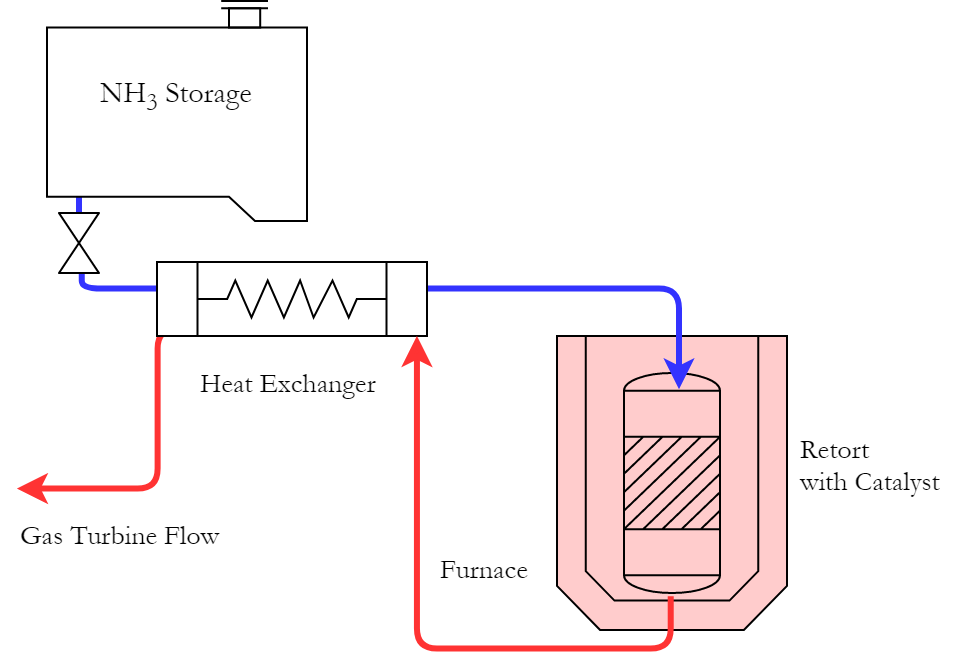
\includegraphics[scale=0.22]{ammonia_cracker}
	\end{figure}}

Due to the high peak demands of the 3 gas turbines a small amount of storage of the cracked gas is stored in order to ensure there is sufficient capacity to meet short term spikes. This is 300 times less than the capacity of the ammonia storage tank. This is done to reduce the capacity requirement of the cracker. The standard capacity of a industrial cracker is 1000 m$^3$/h at operating conditions the plant would require 26 SINCE-GAS ANH units  at a cost of \$6000 per unit \cite{SinceGas2018}. 
\begin{table}[!htbp]
	\begin{center}
		\caption{Ammonia cracker design requirements}
		\begin{tabular}{ |p{7cm}|p{4.5cm}|  }
			
			\hline
			Peak NH$_3$ mass flow demand & 32.815 kg/s\\
			\hline
			Average NH$_3$ mass flow rate required & 0.1648 kg/s\\
			\hline
			Ramp-up time of SOFC&  0.5h\\
			\hline
			Maximum theoretical capacity required& 59067 kg/SOFC ramp-up\\
			\hline
			Minimum turbine down-time    &2h \\
			\hline
			Capacity requirement of cracker& 5.469 kg/s\\
			\hline
			Cracked gas storage requirement & 49.223 ton \\
			\hline
			Total cost of cracker & \$156,000 \\
			\hline
		\end{tabular}
	\end{center}
\end{table}

\subsection{Safety and environmental assessment}

Ammonia synthesis and power generation plants possess a large number of risks associated with them, both in term of their operating conditions but also due to the chemical risks of the materials stored within the plant. 
\\
A recent history has shown that over the past 50 years whilst the rate fires within an ammonia synthesis plant has decreased over time, it remains nontheless a major risk \cite{Ojha2010}\cite{Williams1999}.
\\
A number of studies and risk reviews have been conducted over the past 50 years on the operation and source of risks and failure within Ammonia synthesis plants. In INSERT SOURCE the individual process components are analysed and the major risks are identified for causing serious incident.
\\
\subsubsection{Chemical risk and hazards}
Easily the two most high risk elements of the process are associated with hydrogen and ammonia storage and synthesis. This is due to both the conditions of the process and the chemical effects of the compounds. 
\\
In the case of hydrogen, the main risk associate with it is in storage of high quantities of compressed gas. This is due to the risk of explosion of hydrogen gas under high temperature and pressure. The first method in which to manage this risk is through pressure relief valves in to prevent overpressurization and allow the release of gases before fracture of the storage vessel. However, whilst this prevents the overpressurization within the storage vessels, the formation of hydrogen gas clouds can become present in certain atmospheric conditions and this adequate monitoring of any valve flow must be made and subsequent ventilation of the outlet gas. 
\\
Ammonia has a number of chemical effects whilst it is not considered a  flammable hazardous product due to its high autoignition temperature (651 \textdegree C) and a explosive limit of 16-25\% SOURCE HERE, the first of these being its corrosivity to many metals and alloys including copper and zinc, this means that any storage, piping or fittings to come into contact with ammonia should be made only from Iron and Steel as these do not suffer from the corrosivity on contact of other metals.
\\
Despite its lower density than air evidence suggests that the formation of ammonia gas clouds at ground level is possible in certain environmental conditions \cite{Griffiths1982}. These are largely dependent on wind speed and humidity. Furthermore, despite the possibility of large ammonia clouds forming after a matter of hours the airborne ammonia concentration can change significantly, giving a poor indication of the concentration during the initial release [SOURCE].
\\
The impact of such releases can be varied, and the number of fatalities does not appear to correlate strongly to the amount of ammonia released. A 1400 ton release of ammonia in Lithuania (1989), the largest ever recorded, resulted in a 400km2 affected area and a fatality rate of 7 people, whilst a 38 ton release of ammonia in South Africa (1973) resulted in 18 fatalities,  the highest recorded involving ammonia. This was due to the proximity of a urban population, the speed of ammonia release - caused by brittle fracture - and the environmental conditions at the time - low wind in the direction of the human population. 
\\
Gaseous ammonia can cause severe irritation to the eyes, nose throat and lungs at high enough concentrations whilst contact with liquid ammonia can cause cryogenic burns. The main hazards associated with the levels of toxicity of ammonia and the associated levels of ammonia associated with each hazard is presented in a table below.
\\

\begin{table}[!htbp]
	\begin{center} 
		\caption{SOURCE}
		
		\begin{tabular}{ |p{9.5cm}||p{3.7cm}|  }
			\hline
			Hazard & Concentration (PPM)\\
			\hline
			Threshold limit value (TLV) & 25\\
			Short term exposure limit (STEL)& 35\\
			Immediately dangerous to life and health (IDLH)&300 \\
			Severe eye and respiratory irritation. Permanent damage  &400-700\\
			Convulsive coughing and bronchial spasms &1700\\
			Life threatening   &2500 \\
			Death from suffocation  &5000-10000 \\
			\hline
		\end{tabular}
	\end{center}
\end{table}


Further information on the impact of exposure to ammonia can be found in the Acute Exposure Guideline Levels (AEGS) \cite{Michaels1998}.

When considering methods in which to minimise the hazards caused by ammonia release into the surroundings, a number of methods are available to reduce the risk of a the formation of a high concentration release of ammonia cloud forming. The first of these is the location of the discharge valve. If positioned sufficiently high above ground level the distance travelled to ground level is sufficiently far to allow any high concentrations releases of ammonia to dilute before it reaches the ground, preventing a cloud at ground level forming. Furthermore, the installation of a mist extractor prevents liquid droplets of ammonia being released into the atmosphere. This is especially important due to the highly toxic nature of ammonia on  water ecosystems, as was the case in Arkansas, USA (1971) when a 600 ton spill resulted in the death of thousands of fish on contact with a watercourse, despite no human fatalities \cite{Ojha2010}. 
\\
Whilst a number of methods of managing ammonia and hydrogen release into the atmosphere have been mentioned, the most effective way of minimising the risks associated with ammonia and hydrogen gas is to limit the amount released by normal operation of the plant. This is done by recycling both the purge stream and the vented gas stream from cold storage ammonia. This is done by a reliquification feedback loop.
\\
In the case of the purge a membrane unit under a pressure gradient  is used to separate the hydrogen from the purge so that it can be recovered and added back into the hydrogen feed. In the ammonia vented case it is passed through a flash tank and condenser before being re added to the liquid ammonia tank.
\\
In regard to the location of the ammonia storage tank, it must be placed outside of any plant buildings and at away from any densely populated urban areas and clear of any combustible materials. Furthermore, the storage tank will be at least 100m from any open water storage tank or source of potable water. And any storage location must be easily accessible by road to emergency vehicles and personnel. During any time at which the site is unattended constant monitoring of all liquid and vapour levels must take place whilst any valves with the exception of emergency pressure relief valves must be capped.
\newpage
{\renewcommand{\arraystretch}{0.95}
\begin{landscape}
\begin{table}
	\centering
	\caption{HAZOP analysis of synthesis stage}
	\begin{tabular}{|p{2.65cm}|p{1.4cm}|p{5.7cm}|p{5.2cm}|p{8.2cm}|} 
		\hline
	Line           &Deviation& Cause                                                                                                 & Consequences                                                             & Action                                                                                                                             \\ 
	\hline
	Reactor        & No        & Valve stuck/blocked                                                                                   & Rapid temperature change, Catalyst damage, Reaction rate fall.~          & Measure temperature with a thermocouple and flow rate continuously with alarm and shut down system, catalytic testing.~            \\ 
	\hline
	& Less      & \begin{tabular}[c]{@{}l@{}}Low output concentration,\\Reactor leakage,\\Temperature fall\end{tabular} & Release of reactants, fall in output                                     & Measure concentrations of gases outside of the reactor to detect any leakage of reactants. Catalyst replacement.                   \\ 
	\hline
	& More      & \begin{tabular}[c]{@{}l@{}}Overpressure\\Overtemperature\end{tabular}                                 & Vessel failure, release of reactor gases.                                & Pressure and temperature sensors and warnings, complete shutdown at system before critical level reached. Alarm system in place.~  \\ 
	\hline
	Heat Exchanger & No        & Valve stuck, blockage                                                                                 & Pipe burst - gas leak                                                    & Flow path redundancy in HX.~                                                                                                       \\ 
	\hline
	& Less      & Low heat exchange - damage to surface plate, low flow rate.                                           & Fall in output, damage to HX.                                            & Thermocouple to measure temperature profile of flow. Regular maintenance.                                                          \\ 
	\hline
	& More      & High flow rate, high temperature                                                                      & Overheating of reactor.                                  & Measure flow temperature. Regular maintenance.                                                                                  \\ 
	\hline
	Compressor     & No        & No flow - pump blockage, no power supply, complete pressure loss - leak of compressor                 & Gas leak into atmosphere, reduction in reaction conversion               & Gas monitoring outside chamber, regular maintenance.                                                                               \\ 
	\hline
	& Less      & Low compression level - low power supply/blockage in system                                           & Inefficient operation, damage to pump.                                   & Filter of feed, flow rate and pressure monitoring.                                                                                 \\ 
	\hline
	& More      & Overcompression, power surge, control failure, high flow rate                                         & Damage to compressor pump, pipe rupture. & Power buffer systems. Warning and detection alarms.                                                                                \\ 
	\hline
	Separator      & No        & No output flow - separator leak                                                                       & No ammonia output, gas leak                                              & Continuous monitoring of pressure, temperature and flow rates. Regular inspection.                                                 \\ 
	\hline
	& Less      & Temperature too high                                                                                  & Mesh damage, low yield.                                       & Regular stream testing. Periodic inspection.                                                                  \\ 
	\hline
	& More      & Temperature too low                                                                                   & Power wastage in cooling.                                        & Thermocouple to measure vessel temperature.                                                                                 \\ 
	\hline
	Storage        & No        & No~                                                                                                   & Failure power generation stages                         & Monitoring of storage levels, low storage warning.                                                                                 \\ 
	\hline
	& Less      & Refrigeration failure of vessel                                                                       & Building up of pressure - burst vessel                                   & Leak before burst design of storage tank. Pressure relief valve.~                                                                  \\ 
	\hline
	& More      & Buildup of pressure in container - failure of gas release valve                                       & Vessel failure/bursting                                                  & Redundancy in~ release valves, regular inspection. Pressure monitoring inside vessel.                                              \\
	\hline
	\end{tabular}
\end{table}
\end{landscape}
}
\newpage


\subsection{Economic assessment}
An economic analysis of the requires an assessment of the costs associated with each stage of the design.
\newpage
\subsection{Results and process summary}
During the final design iteration of the synthesis stage a first pass conversion rate of \conv \% can be achieved after optimization. This is achieved at a pressure of \pbar  bar and a reactor inlet temperature of \tc\textdegree C. Figure \ref{aspenF} shows the final stage ammonia synthesis stage ASPEN flow diagram. 
{\centering
	\begin{figure}[h]
		\caption{ASPEN model of synthesis reaction}
		\label{aspenF}
		
		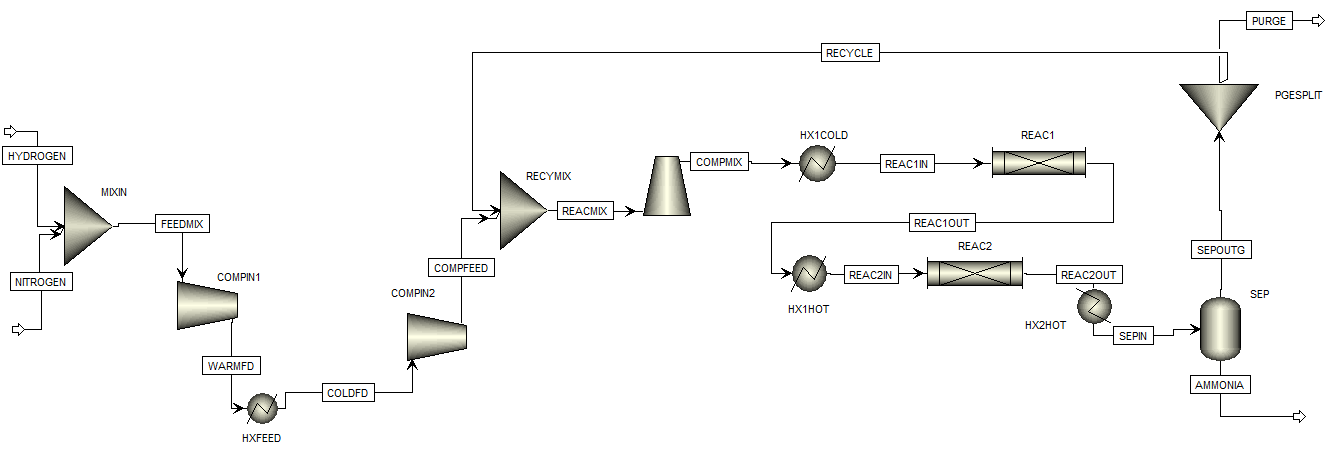
\includegraphics[scale=0.48]{ASPEN_MODEL}
		
\end{figure}}
 
 The ammonia synthesis, whilst a well established process requires careful design and optimisation of the process due to the specific design requirements. The use of ASPEN and MATLAB has allowed for the creation of a dynamic modelling system that has enabled the conversion rate of ammonia within the reactor to be optimised, whilst design of the ammonia storage requirements and power generation needs of the plant have enabled the output of this stage to be designed to minimise the waste output of the plant through stream recycles.

%\printbibliography[heading=subbibliography]
\bibliography{./ammoniasynth/v3bib}
\bibliographystyle{unsrt}
%\end{document}